\documentclass[12pt]{extarticle}
\usepackage[english, russian]{babel}
\usepackage[left=20mm, right=10mm, top=20mm, bottom=20mm]{geometry}
\usepackage{graphicx}
\usepackage{titlesec}
\usepackage{array}
\usepackage{wrapfig}
\usepackage{color, colortbl}
\usepackage[colorlinks=true,linkcolor=cyan,unicode=true]{hyperref}
\usepackage{mathtools}
\usepackage{setspace}
\usepackage{svg}
\usepackage{amssymb}
\usepackage{makecell}
 
\newcommand\ddformula[1]{\displaystyle #1}
 
\titleformat{\section}
  {\normalfont\fontsize{12}{14}\bfseries}{\thesection}{0.5em}{}
 
\begin{document}
    \begin{minipage}{0.5\textwidth}
        \begin{center}
            \begin{small}
                \textsf{\textbf{Университет ИТМО}} \\
                \textsf{\textbf{Факультет программной инженерии и}} \\
                \textsf{\textbf{компьютерной техники}}
            \end{small}
        \end{center}
    \end{minipage}
    \hfill
    \begin{minipage}{0.4\textwidth}
        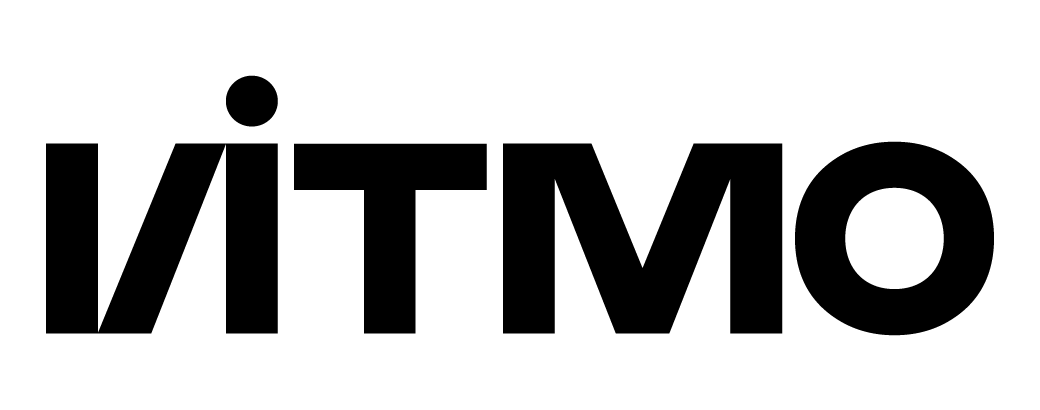
\includegraphics[height=2.5cm]{itmo.png}
    \end{minipage}
    \hrule
    \vspace{8mm}
    \begin{minipage}{0.4\textwidth}
        Группа: P3215 \\ % ГРУППА
        Студент: Барсуков М.А. \\ % СТУДЕНТ
        Преподаватель: Смирнов А.В % ПРЕПОД
    \end{minipage}
    \hfill
    \begin{minipage}{0.4\textwidth}
        К работе допущен: \\
        Работа выполнена: \\
        Отчёт принят: 
    \end{minipage}
    \vspace{8mm}
    \begin{center}
        \begin{Large}
            \textbf{Рабочий протокол и отчёт по лабораторной работе №3.01} \\ % УКАЗАТЬ НОМЕР ЛАБЫ
            Изучение электростатического поля методом моделирования % УКАЗАТЬ НАЗВАНИЕ ЛАБЫ
        \end{Large}
    \end{center}
    \vspace{8mm}
 
    \section{Цель работы}
    Изучить электростатическое поле, построив сечения эквипотенциальных поверхностей и силовых линий электростатического поля на основе экспериментального моделирования распределения потенциала в слабопроводящей среде

    \section{Задачи, решаемые при выполнении работы}
    1. Изобразить данные измерений на масштабно-координатную бумагу
    \\2. Построить сечения эквипотенциальных поверхностей и силовых линий электростатического поля
    \\3. Проанализовать данные
    \\4. Провести косвенные вычисления
    \\5. Построить графики зависимостей $\varphi = \varphi(x)$
    
    \section{Объект исследования}
    Потенциал в слабопроводящей среде

    \section{Метод экспериментального исследования}
    Эксперимент. Размещение в слабопроводящей среде электродов для построения сечений эквипотенциальных поверхностей и силовых линий

    \newpage
    \section{Рабочие формулы и исходные данные}
    
    Средняя напряженность
    \begin{equation*}
        \langle E_{12} \rangle \approxeq \frac{\varphi_1 - \varphi_2}{l_{12}}
    \end{equation*}
    где $l_{12}$ - длина участка силовой линии между точками, 
    $\varphi_1$ и $\varphi_2$ потенциалы двух точек, лежащих на одной силовой линии \\
   Поверхностная плотность на электродах: \\
   \begin{equation*}
        \sigma^\prime \approxeq -\varepsilon_0\frac{\Delta\varphi}{\Delta l_n}
   \end{equation*}
   где $\Delta\varphi$ - изменение потенциала при смещении на малое расстояние $\Delta l_n$ по нормали к поверхности проводника, 
   $\varepsilon_0 \simeq 8.85 * 10^{-12} \frac{\text{Ф}}{\text{м}}$ - электрическая постоянная
    \section{Измерительные приборы}
    \begin{tabular}{|p{1cm}|p{4cm}|p{5cm}|p{32mm}|p{3cm}|}
        \hline
        \textbf{№} & \textbf{Наименование} & \textbf{Тип прибора} & \makecell{\textbf{Используемый}\\\textbf{диапазон}} & \makecell{\textbf{Погрешность}\\\textbf{прибора}} \\ \hline
        1 & Вольтметр & Измерение потенциала & 0 - 20 В & 0.1 В \\ \hline
        2 & Линейка & Ось абцисс & 2-28 см & 1 мм \\ \hline
        3 & линейка & Ось ординат & 2-18 см & 1 мм \\
        \hline
    \end{tabular}
    
    \section{Схема установки}
    \begin{minipage}{0.5\textwidth}
        \includegraphics[height=7cm]{image0.png}
    \end{minipage}
    \hfill
    \begin{minipage}{0.4\textwidth}
        На боковых стенках электролитичtской ванны
        расположены плоские металлические электроды,
        подключенные к многофункциональному генератору напряжения ГН1.
        Между электродами находится измерительный зонд в виде 
        тонкого изолированного проводника, подсоединенного к вольтметру.
        Вольтметр в составе комбинированного прибора АВ1 показывает
        действующую разность потенциалов между зондом и электродом,
        подключенным ко второму гнезду вольтметра. Собственное 
        сопротивление вольтметра существенно превышает сопротивление
        воды в ванне, для того чтобы измерительный ток вольтметра не
        шунтировал токи в модели и не искажал распределение электрического поля
    \end{minipage}

    \newpage
    \section{Результаты прямых измерений}
    \includegraphics[height=18cm,angle=90]{right.jpg}
    \section{Результаты косвенных измерений}
    \begin{equation*}
        E_{min} = \frac{\varphi_2 - \varphi_1}{l_{12}} = 0
    \end{equation*}
    \begin{equation*}
        E_{max} = \frac{\varphi_2 - \varphi_1}{l_{12}} = 58.824
    \end{equation*}
    Напряженность возле одного из электродов
    \begin{equation*}
        E = \frac{4 - 2}{0.046} = 43.478
    \end{equation*}
    Поверхностная плотность на электродах
    \begin{equation*}
        \sigma^\prime = -3.85 * 10^{-10} \frac{\text{Кл}}{\text{м}^2}
    \end{equation*}
    \textbf{Распределение напряженности} \\
    \begin{tabular}{|p{3cm}|p{3cm}|p{3cm}|p{3cm}|p{3cm}|}
        \hline
        43,478 & 40,816 & 37,037 & 39,216 & 40,816 \\ \hline
        45,455 & 42,553 & 34,483 & 40,816 & 44,444 \\ \hline
        48,78  & 48,78  & 27,397 & 46,512 & 48,78  \\ \hline
        51,282 & 55,556 & 23,529 & 54,054 & 50          \\ \hline 
        51,282 & 50     & 23,529 & 58,824 & 52,631 \\ \hline
        48,78  & 57,143 & 23,529 & 54,054 & 51,282 \\ \hline
        46,512 & 51,282 & 27,397 & 47,619 & 47,619 \\ \hline
        42,553 & 43,478 & 34,482 & 42,553 & 46,512 \\ \hline
        38,462 & 40,816 & 39,216 & 42,553 & 40,816 \\ \hline
    \end{tabular}
    
    \section*{Расчёт погрешностей измерений}
    $\Delta \varphi = 0.1\text{В}$ \\
    $\Delta x = 0.001 \text{м}$
    \begin{equation*}
        \Delta E = \sqrt{(\frac{\delta(\frac{\varphi_2 - \varphi_1}{l_{12}})}{\delta\varphi_1}\Delta\varphi_1)^2
         + (\frac{\delta(\frac{\varphi_2 - \varphi_1}{l_{12}})}{\delta\varphi_2}\Delta\varphi_2)^2
         + (\frac{\delta(\frac{\varphi_2 - \varphi_1}{l_{12}})}{\delta l_{12}}\Delta l_{12})^2} =
         \sqrt{2(\frac{\Delta\varphi}{l})^2 + (\frac{\varphi_2 - \varphi_1}{l^2}\Delta l)^2}
    \end{equation*}
    $\Delta E = 3.216$
    \begin{equation*}
        \Delta\sigma^\prime = \varepsilon_0\sqrt{(\frac{\Delta\varphi}{l})^2 + (\frac{\varphi_2 - \varphi_1}{l^2}\Delta l)^2} = 
    \end{equation*}
    $\Delta\sigma^\prime = 2.098 * 10^{-12}$
    \section{Графики}
    \includegraphics[height=11cm]{image1.png}

    \section{Вывод и анализ результатов}
    В ходе лабораторной работы было выявлено, что самые высокие значения напряжённости электрического поля наблюдаются вокруг проводника, в то время как самые низкие значения фиксируются непосредственно в области проводника. Максимальная напряжённость была зарегистрирована в области кончика стрелки.\\
Эти результаты позволяют сделать несколько ключевых выводов. Во-первых, высокая напряжённость вокруг проводника указывает на концентрацию силовых линий электрического поля вблизи проводящей поверхности. Это явление соответствует теоретическим ожиданиям, так как силовые линии стремятся перпендикулярно выходить из поверхности заряженного проводника и максимально концентрируются на остриях и неровностях, что объясняет максимальную напряжённость у кончика стрелки.\\
Во-вторых, низкие значения напряжённости в области проводника свидетельствуют о том, что внутри проводника электрическое поле практически отсутствует. Это связано с тем, что в проводнике свободные заряды перераспределяются таким образом, чтобы внутреннее электрическое поле компенсировалось, приводя к нулевому значению внутри проводника.\\

    \newpage
    \includegraphics[height=25cm]{back.jpg}
    \end{document} 